\documentclass[UTF8]{ctexart}

% 本模版示范和环境载入部分可以用第一行的收缩键把示范收缩掉,需要的时候再打开。从40行开始进行示范。

% 更改页边距
\usepackage[left=2.5cm,right=2.5cm,top=2.5cm,bottom=2.5cm]{geometry}

% 设置引用
\usepackage[utf8]{inputenc}
\usepackage{url}
\usepackage{hyperref}

\usepackage{graphicx}
\usepackage{adjustbox}
\usepackage{caption}
\usepackage{amsmath} % 数学公式
\usepackage{amssymb} % 符号引入
\usepackage{hhline}

% 长注释
\usepackage{comment}
\begin{comment}
    这里是一个长注释。
\end{comment}

% 为公式自动编号
\makeatletter
\@addtoreset{equation}{section}
\makeatother
\renewcommand{\theequation}{\arabic{section}.\arabic{equation}}

\setcounter{tocdepth}{3} % 控制目录深度

\title{Text Similarity from Time Series Perspective}
\author{
    范维
}
% \date{2024年5月28日}
\date{\today}


% 大段示范

% 1. 可调节大小的表格和引用
% \ref{tab:example}
% \nameref{tab:example}
% \begin{table}[htbp]
%     \captionsetup{position=top, skip=8pt}
%     \caption{表格标题}
%     \centering
%     \begin{adjustbox}{width=0.5\textwidth}
%         \begin{tabular}{c|c|c}
%             \hline
%             \textbf{\small 姓名} & \textbf{\small 学号} & \textbf{\small 成绩}  \\
%             \hline
%             \small winston & \small 1111111 & \small 1111111   \\
%             \hline
%             \small hello & \small 2222222 & \small 1111111     \\
%             \hline
%             \small Amy & \small 3333333 & \small 1111111       \\
%             \hline
%         \end{tabular}
%     \end{adjustbox}
%     \label{tab:example}
% \end{table}

% 2. 不自动排版的图片和引用
% \ref{fig:pic}
% \nameref{fig:pic}
% \begin{figure}[htbp]
%     \captionsetup{position=bottom, skip=8pt}
% 	\centering
% 	\includegraphics[width=0.5\textwidth]{image_url_not_include_png}
%     \caption{图片标题}
% 	\label{fig:pic}
% \end{figure}

% 3. 文献引用
% \cite{ref1} 引用一篇文章
% \begin{thebibliography}{99}

%     \bibitem{ref1} Kingma, D. P., \& Ba, J. (2014, December 22). Adam: A Method for Stochastic Optimization. ArXiv.Org. \url{https://arxiv.org/abs/1412.6980v9}

% \end{thebibliography}

% 4. 文字中套公式和引用
% 带括号引用\eqref{eq:eg} 不带括号引用\ref{eq:eg}
% {
% 	We can use $公式$ to solve the equations.
% 	Or we can use matrix equation
% 	\begin{gather}
% 		\pi_{i-1}(t) \notag \\
%       \text{If we have } \pi_{i-1}(t) \label{eq:eg}
% 	\end{gather}
% }

% 5. 列表

% 有序
% \begin{enumerate}
%     \item 第一项
% \end{enumerate}

% 无序
% \begin{itemize}
%     \item 第一项
% \end{itemize}

% 6. 大括号

% 左侧大括号
% \begin{gather}
% 	\left\{
% 	\begin{array}{ll}
% 		\dot{\pi_0(t)} = \mu \pi_1(t)                              \\
% 		\dot{\pi_1(t)} = 2\mu \pi_2(t) - \mu \pi_1(t)              \\
% 		\dot{\pi_2(t)} = 3\mu \pi_3(t) - 2\mu \pi_2(t)             \\
% 		\text{\quad\quad\quad\quad}\vdots                          \\
% 		\dot{\pi_i(t)} = (i+1)\mu \pi_{i+1}(t) - i\mu \pi_{i}(t) \\
% 		\text{\quad\quad\quad\quad}\vdots                          \\
% 		\dot{\pi_N(t)} = -N\mu \pi_N(t)
% 	\end{array}
% 	\right. \notag
% \end{gather}

% 上方大括号
% \begin{gather}
%     \dot{\pi_0(t)} = \overbrace{[\mu_2 \pi_3(t)]}^{\text{into}} - \overbrace{[\lambda \pi_0(t)]}^{\text{outof}}
% \end{gather}

% 7. 矩阵
% \[ \mathbf{Q} = \left(
%     \begin{array}{ccccc}
%             -\lambda & \lambda  & 0        & 0        & \ldots \\
%             0        & -\lambda & \lambda  & 0        & \ldots \\
%             0        & 0        & -\lambda & \lambda  & \ldots \\
%             0        & 0        & 0        & -\lambda & \ldots \\
%             \vdots   & \vdots   & \vdots   & \vdots   & \ddots \\
%         \end{array} \right) \]

% 8. 自定义命令
% \newcommand{\myeqref}[1]{公式 \eqref{#1}}


% 正文开始

\begin{document}

% 封面
\pagestyle{empty} % 设置封面不显示页号
\vspace*{12em} % 垂直间距
% 标题
\begin{center}
    {\Huge Text Similarity from Time Series Perspective}\\
    \bigskip
    \bigskip
    {\LARGE 高级商务智能 \quad 期末项目}
\end{center}
\vspace{12em} % 垂直间距

% 信息
\begin{center}
    {\Large
        \begin{tabular}{rl}
            姓名: & \underline{\makebox[10em][c]{范维}}         \\
            学号: & \underline{\makebox[10em][c]{2023214429}} \\
            班级: & \underline{\makebox[10em][c]{信息管理与商务智能}}  \\
        \end{tabular}
    }
\end{center}

\clearpage  % 这一页结束后,页码重新开始

\tableofcontents % 目录
\clearpage

\pagestyle{plain}
\maketitle

\section{Abstract}
 {
  This paper focuses on the task of measuring text similarity.\footnote{The code is hosted in the library \url{https://github.com/WinstonFanWei/TextSimilarity}.}
  Traditional methods for text similarity, such as the Bag-of-Words model, rarely consider the order of words in the text,
  which can lead to inaccurate similarity measures.
  Our approach transforms text information into word or sentence representation vectors using models like Word2Vec,
  and then views these representation tensors from a time series perspective.
  By employing Dynamic Time Warping (DTW) \cite{ref1},
  we calculate the distance between texts and convert this distance into a similarity measure.
  This method takes into full account the order of words and sentences,
  providing a more accurate measurement of text similarity.
  We designed unsupervised experiments to measure similarity and compared our results with expert human ratings across various dimensions.
  Our model demonstrated promising performance.
  In the future, we may improve the text embedding model and develop a supervised prediction model to further enhance prediction accuracy.
 }
\newpage

\section{Introduction}
 {
  The accurate measurement of text similarity is a critical task in Natural Language Processing (NLP) with applications spanning information retrieval, document clustering, plagiarism detection, and semantic search. Traditional methods for text similarity, such as the Bag-of-Words (BoW) model, are limited by their disregard for the sequential nature of text, which often leads to inaccurate similarity assessments.

  Most text similarity measurements convert two texts into highly summarized vectors using models, then calculate their similarity by computing the cosine similarity of these vectors. The Bag-of-Words (BoW) model simplifies text to a collection of word frequencies, ignoring word order and context. Models like TF-IDF and LDA, which are based on the BoW model, share the same issue.

    Although models such as Word2Vec \cite{ref2} consider word order when generating word embedding vectors, they do not fully utilize global word order information during the final comparison of document similarities. The Word Mover's Distance (WMD) model improves similarity calculations by aligning words in the texts, but it also overlooks word order.

    In the time series perspective, we already have methods to measure similarity. By representing text as a time series and applying these methods, we can account for word order information, an approach that has been largely overlooked.

    This modeling approach allows us to represent text as a matrix of word vectors, directly feeding the lowest-level text representation into the model, potentially enhancing its performance. Unlike structural methods in NLP that require assumptions about and learning the parameters of the generative process, viewing text as a time series enables similarity calculations through alignment without these assumptions.

    
    Therefore, our alignment approach has many advantages over the traditional structural approach, which summarizes document semantics into a vector by training generative language models.

  To address these limitations, we propose an innovative approach that leverages advanced text representation techniques and sequence alignment methods. Specifically, we transform text information into word or sentence representation vectors using models like Word2Vec. These vectors are then analyzed from a time series perspective, allowing us to apply Dynamic Time Warping (DTW) \cite{ref1} to measure the distance between texts. This method preserves the order of words and sentences, thereby providing a more accurate measurement of text similarity.

  Our experimental setup involves a comprehensive analysis using a legal document dataset\footnote{The same dataset as that metioned in \cite{ref3}.}, consisting of 144 legal documents and an accompanying Excel file with 100 expert-annotated similarity scores. The experiments were designed to compare the performance of different similarity measurement methods:

    \newpage

  \begin{enumerate}
      \item Method 1: We used TF-IDF \cite{ref4} to create a BoW model and computed similarity using cosine similarity.
      \item Method 2: Each document was modeled using a pre-trained Latent Dirichlet Allocation (LDA) \cite{ref5} model to obtain topic distribution vectors. Document similarity was then computed using cosine similarity on these vectors.
      \item Method 3: At the word or sentence level, documents were modeled using LDA. We measured topic distance by considering the distribution of words or sentences within each topic using word movement distence (WMD) \cite{ref6}. For each document, the topic of each token was determined, and DTW was used to calculate the distance between documents, effectively considering word order information.
  \end{enumerate}

  To evaluate the effectiveness of these methods, we employed various metrics including Root Mean Squared Error (RMSE), F1-score, and correlation with human-annotated scores. Our results demonstrate that the DTW-based method, which incorporates word order information, significantly outperforms traditional methods in aligning with expert human ratings.

  This paper makes several contributions to the field of text similarity measurement. First, we introduce a novel application of DTW to text similarity, which effectively incorporates the sequence of words. Second, we provide empirical evidence through unsupervised experiments that our model aligns well with human judgments across multiple dimensions.

  Looking forward, we plan to enhance our approach by refining the text embedding models and developing supervised prediction models to further improve prediction accuracy. This could involve integrating advanced contextualized embeddings, such as those produced by BERT \cite{ref7}, and exploring other alignment techniques that better capture the nuances of textual data.
 }

 \newpage

\section{Related Work}
 {
  In the realm of text similarity measurement, traditional approaches have been extensively surveyed by (H.Gomaa \& A. Fahmy, 2013)\cite{ref8}. They categorize these approaches into three main types: String-Based, Corpus-Based, and Knowledge-Based methods. String-Based methods focus on character and term matching, such as the Longest Common Substring and Cosine Similarity. Corpus-Based methods utilize large text corpora to derive semantic relationships, exemplified by Latent Semantic Analysis (LSA) and Explicit Semantic Analysis (ESA). Knowledge-Based methods leverage structured semantic networks like WordNet to assess similarity based on shared meanings and relationships. This comprehensive survey underscores the limitations of conventional methods in capturing the sequential nature of text, which our proposed time series perspective on a Corpus-Based model aims to address.

  (Gong et al., 2018)\cite{ref9} presents a novel approach to matching long documents with their summaries by utilizing hidden topic modeling and domain-specific word embeddings. This method addresses the challenges of vocabulary and context mismatches that arise due to the varying lengths of the texts being compared. The authors propose a multi-view generalization of the document through hidden topics to bridge the gap between detailed texts and their abstractions.

  (Kusner et al., 2015)\cite{ref6} introduces the Word Mover's Distance (WMD), a novel metric for measuring the distance between text documents based on word embeddings. The WMD represents documents as weighted point clouds of embedded words and calculates the minimum cumulative distance that words from one document need to "travel" to match the point cloud of another document. This approach leverages the semantic meaning captured by word embeddings like Word2Vec, which can capture relationships between words. The WMD is shown to be highly effective, outperforming several state-of-the-art document distance metrics in real-world document classification tasks.

  (Matuschek et al., 2008)\cite{ref1} This article introduces a novel approach for comparing typed texts by transforming them into artificial time series and then measuring their similarity using Dynamic Time Warping (DTW) distance. The method involves counting relevant keywords within a sliding window applied to the text to create the time series, which can then be analyzed with time series analysis techniques. The authors demonstrate that this technique is effective for recognizing similar texts, including those in different languages, and could aid in plagiarism detection and information retrieval. They also discuss the potential for further development, such as incorporating additional text preprocessing steps and combining this method with other information retrieval techniques.
 }
\newpage

\section{Model}

\subsection{LDA and Word2Vec}
{
    Latent Dirichlet Allocation (LDA) \cite{ref5} is a generative statistical model, used to identify latent topics within a collection of documents. As \nameref{fig:LDA_1} shows, LDA assumes each document is a mixture of several topics, with each topic being characterized by a distribution over words. By using Dirichlet distributions to model the variability of topic proportions per document and word distributions per topic, LDA can infer the hidden topic structure from the observed words. This inference typically involves techniques like Variational Bayes or Gibbs Sampling.

    \begin{figure}[htbp]
        \captionsetup{position=bottom, skip=8pt}
        \centering
        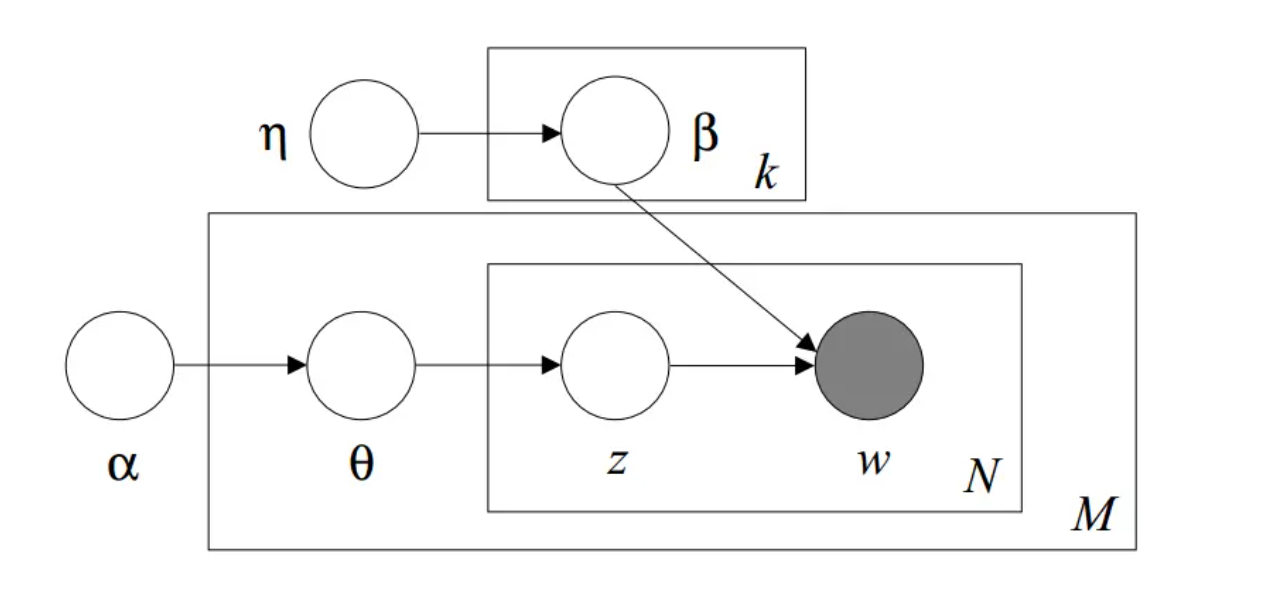
\includegraphics[width=0.6\textwidth]{LDA_1}
        \caption{Probabilistic graphical model of LDA}
        \label{fig:LDA_1}
    \end{figure}

    We use LDA to model the probability distribution of words in each topic and the probability distribution of topics in each document, which can then be used in TS-DS and other models.

    Word2Vec \cite{ref2} is a popular unsupervised learning algorithm that learns word embeddings from a large corpus of text. As \nameref{fig:Word2Vec_1} shows, it is based on the skip-gram model, which predicts the context words given the target word, and the continuous bag-of-words model, which predicts the target word given the context words.

    \begin{figure}[htbp]
        \captionsetup{position=bottom, skip=8pt}
        \centering
        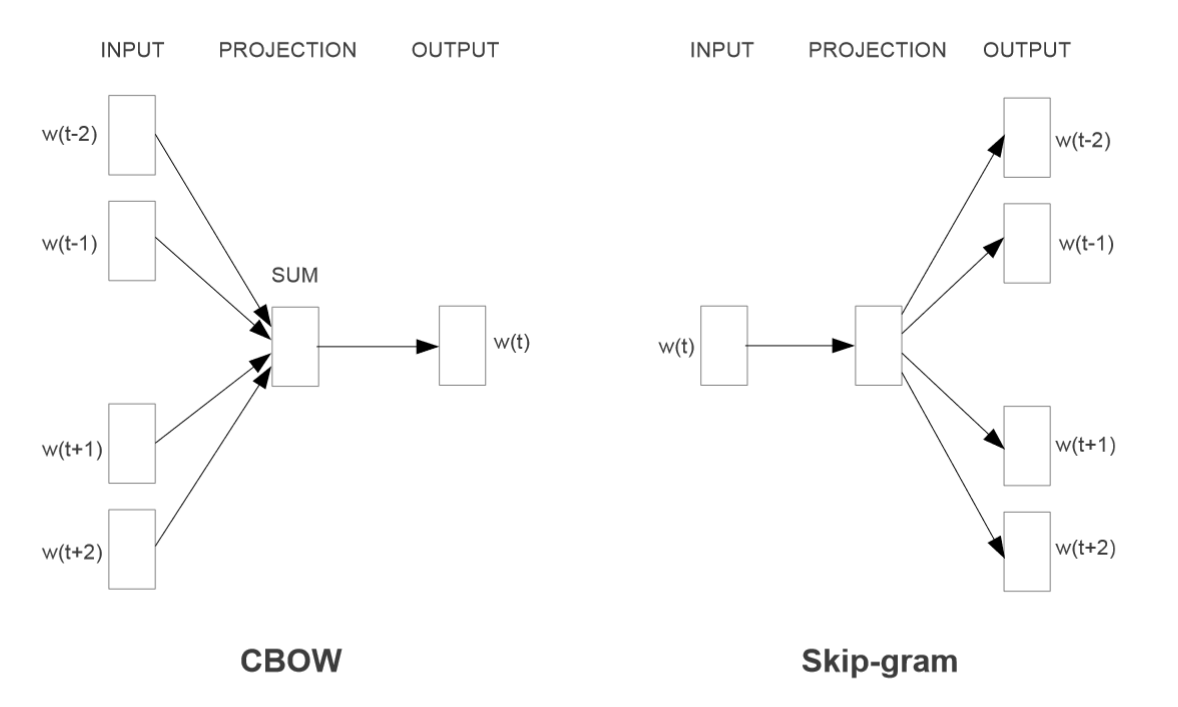
\includegraphics[width=0.5\textwidth]{Word2Vec_1}
        \caption{Word2Vec architectures}
        \label{fig:Word2Vec_1}
    \end{figure}

    We use Word2Vec to generate word embeddings for each word in the corpus, which can then be used to represent the documents in the latent space.
}

\subsection{Measure Document Similarity from Time Series Perspective(TS-DS)}
{
    As \nameref{fig:TS_DS} illustrates,
    the TS-DS model first uses the word2vec model to embed every word that appears in the entire document collection.
    By calculating the distances between these word embeddings, we obtain the distances between words. Simultaneously,
    LDA is used to model the entire document collection, yielding the word distributions for each topic.
    Subsequently, using each topic's word distribution and the distances between words,
    we can calculate the Word Mover's Distance (WMD) between topics.
    Finally, we represent each document as a sequence of topics,
    where each position corresponds to the most probable topic for each word in the document.
    We then use Dynamic Time Warping (DTW) to calculate the distances between the topic sequences of each document,
    which is then converted into similarity.

    \begin{figure}[htbp]
        \captionsetup{position=bottom, skip=8pt}
        \centering
        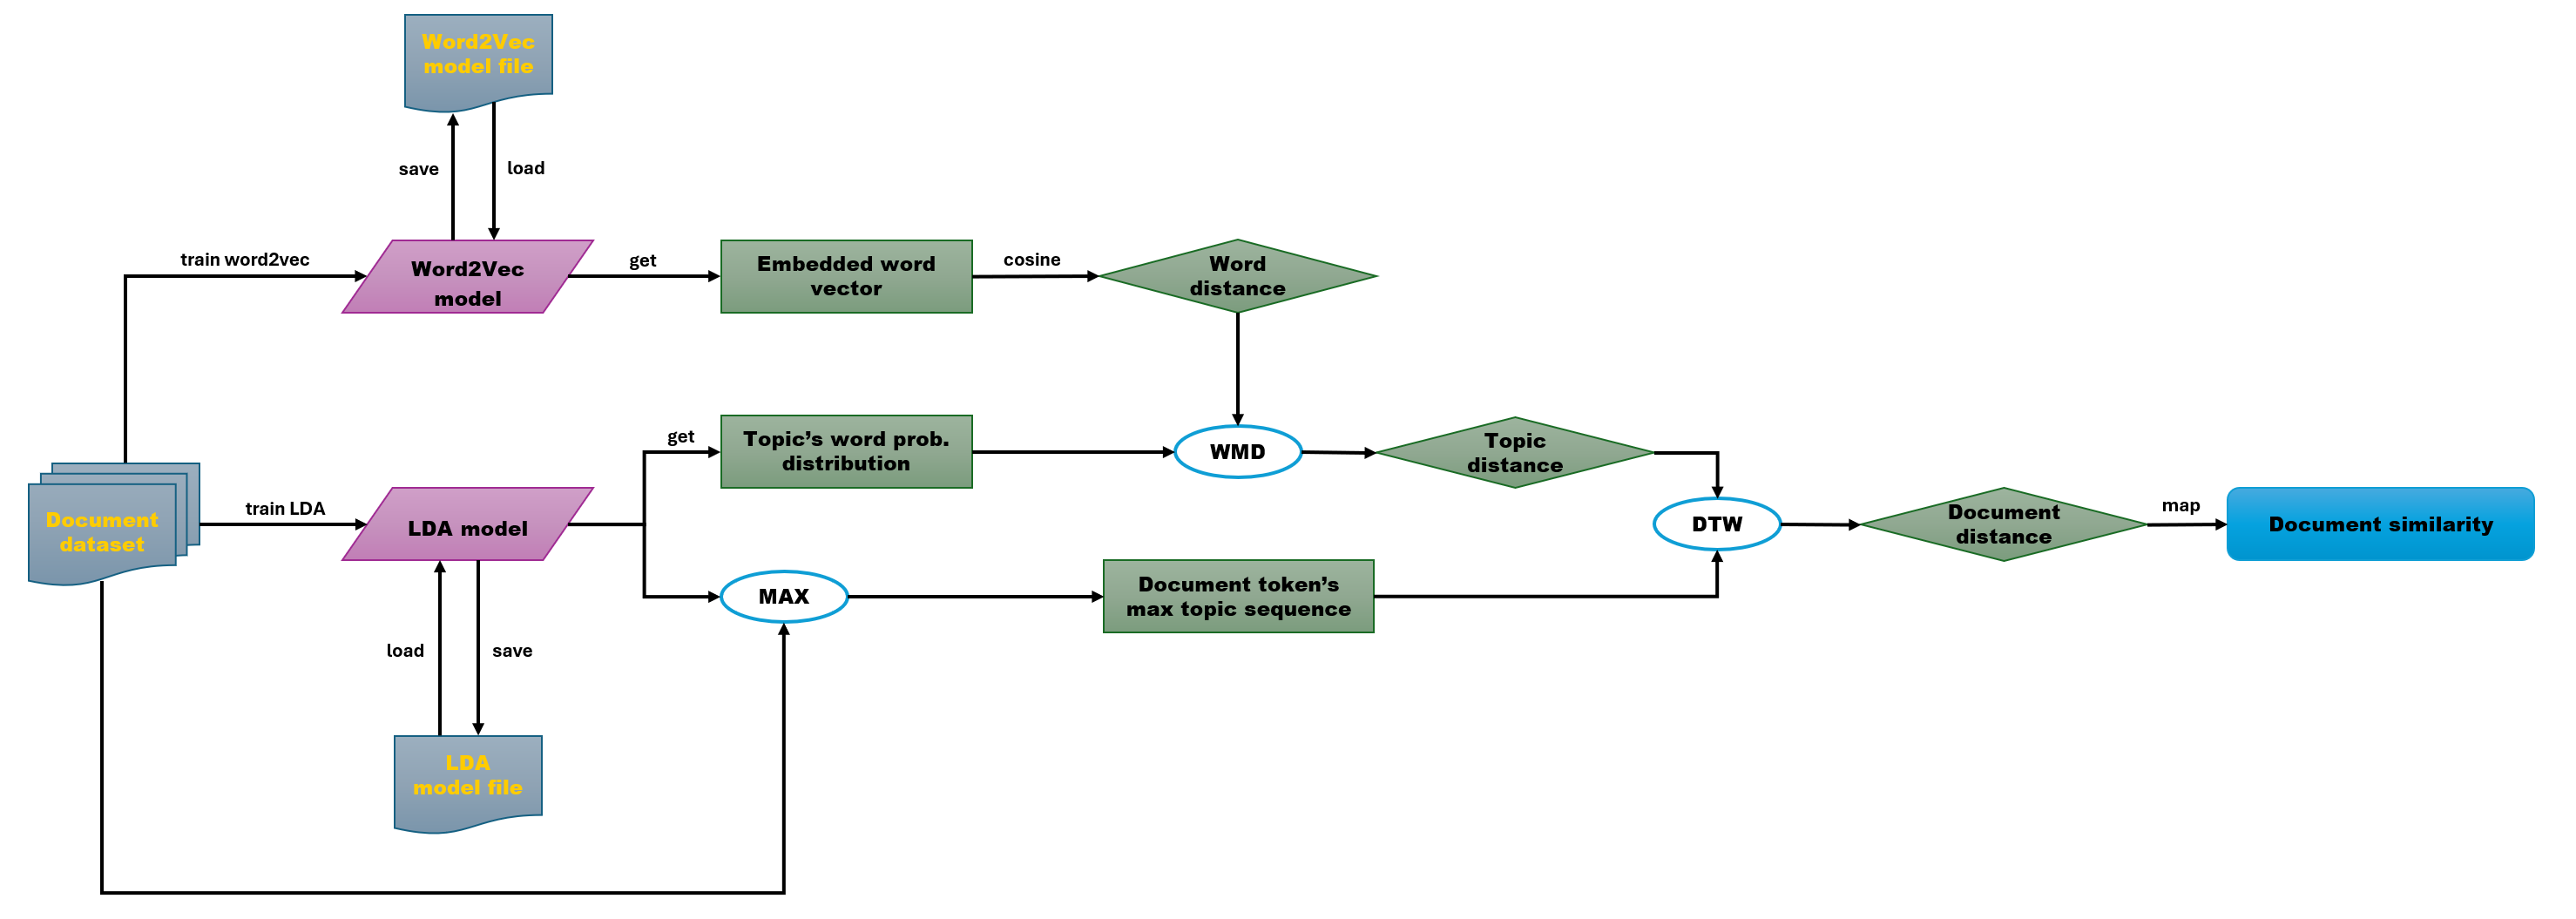
\includegraphics[width=1\textwidth]{TS_DS}
        \caption{The entire TS-DS model}
        \label{fig:TS_DS}
    \end{figure}
}

\subsubsection{Topic distance matrix(TDM)}
{
    "Topic distance" is an intriguing way to measure the semantic and thematic divergence between topics within a corpus. 
    It leverages the power of Word2Vec for generating dense vector representations of words, capturing their semantic relationships. 
    Topic distance is calculated by first determining the distances between individual words using Word2Vec and cosine similarity, 
    and then applying these distances to the word distributions of topics using WMD. 
    This approach allows for a detailed and nuanced comparison of the thematic structures revealed by LDA, 
    where each topic is characterized by a specific distribution of words.

    To compute the topic distance, one begins by embedding words into a continuous vector space using Word2Vec, 
    allowing for a nuanced understanding of word similarities. 
    However, if we calculate the distances between all pairs of words,
    the computational load becomes enormous. Therefore,
    we consider taking measures to reduce the number of words in the corpus, 
    which in turn reduces the cost of computing and storing word similarities. 
    Currently, we use a filter to exclude words that appear less than five times. 
    We then perform cosine comparisons on the remaining word pairs to obtain their similarities and then transfer them to distance by \eqref{eq:D_word}.

    The crux of topic distance lies in comparing word distributions across topics.
    This is achieved by conceptualizing each topic as a probability distribution of words and calculating the distance
    between these distributions, through the Word Mover's Distance (WMD), as \eqref{eq:TDMxy} and \eqref{eq:TDMst} show.

    WMD operates by considering the minimum amount of "work" required to transform one distribution of topic vectors into another. 
    This "work" is quantified as the cumulative distance words from one topic need to "travel" to match the distribution of words in another topic.
    Essentially, it measures how much one topic's word distribution must be altered to resemble another topic's word distribution.
    This method provides a nuanced measure of the thematic dissimilarity between topics,
    capturing subtle differences in word usage and context that might be overlooked by simpler metrics.

    In essence, topic distance is a multi-faceted metric that amalgamates the semantic
    closeness of individual words with the topic composition of words. 
    It offers a comprehensive assessment of topic divergence by considering both the distribution of words within 
    topics and the semantic relatedness of those words. 
    This approach not only enhances our ability to discern the thematic landscape of textual data but also provides 
    a framework for analyzing topic similarity.

    With parameters $Dim := Dimension \hspace{0.1cm} of \hspace{0.1cm} word \hspace{0.1cm} embedding$, $N := Total \hspace{0.1cm} word \hspace{0.1cm} count,$
    \begin{gather}
        WordVec_{i} := (w_i^1, w_i^2, \dots, w_i^{Dim}) \\
        D_{word}^{i, j} = 1 - \frac{WordVec_{i} \times WordVec_{j}}{\left| WordVec_{i} \right| \times \left| WordVec_{j} \right|} \label{eq:D_word} \\
        M := \{D_{word}^{i, j}\}_{N \times N}
    \end{gather}


    For the topic distance matrix $TDM$, we use WMD to determine each element. For example, the distance between topic x and topic y is given as a optimal problem:

    \noindent \rule{\linewidth}{0.2mm}
    \noindent $WMD \hspace{0.2cm} optimal \hspace{0.2cm} problem$:
    \begin{gather}
        TDM_{x, y} = \min_{Q = \{ q(1,1), q(1,2), \dots, q(N,N) \}} \left( \sum_{i \in \{1, \dots, N\}} \left( \sum_{j \in \{1, \dots, N\}} q(i,j) \times M(i,j) \right) \right) \label{eq:TDMxy} \\
        s.t.
        \left\{
        \begin{array}{ll}
            \sum_{j \in \{1, \dots, N\}} q(i,j) = w_{x}^i, \hspace{0.1cm} \forall i \in \{1, \dots, N\} \\
            \sum_{i \in \{1, \dots, N\}} q(i,j) = w_{y}^j, \hspace{0.1cm} \forall j \in \{1, \dots, N\} 
        \end{array}
        \right. \label{eq:TDMst}
    \end{gather}
    \noindent \rule{\linewidth}{0.2mm}

    With parameter $E := Total \hspace{0.1cm} topic \hspace{0.1cm} count,$
    \begin{gather}
        TDM = \{TDM_{i, j}\}_{E \times E} =
        \left(
        \begin{array}{cccc}
                0          & TDM_{1, 2} & TDM_{1, 3} & \ldots \\
                TDM_{1, 2} & 0          & TDM_{2, 3} & \ldots \\
                TDM_{1, 3} & TDM_{2, 3} & 0          & \ldots \\
                \vdots     & \vdots     & \vdots     & \ddots \\
            \end{array}
        \right)_{E \times E} \label{eq:TDM}
    \end{gather}

    We can see from \eqref{eq:TDM} that the TDM matrix is a symmetric matrix with diagonal elements equal to 0. 
    This is because, unlike the calculation of KL divergence \cite{ref10}, 
    the transportation distance from topic x to topic y is equal to the transportation distance from topic y to topic x in WMD. 
    Additionally, if the word probability distributions of the two topics are equal, then the $q(i,j)$ term in \eqref{eq:TDMxy} will always be 0, 
    thus all diagonal elements are 0.
}

\subsubsection{Documents distance from topic series perspective using DTW}
{
    We extract the most likely topic for each word in every document from the LDA model, 
    forming a sequence of topics for each document based on the word order, which is used in \eqref{eq:DTW_distance}.
    By leveraging the distances between topics that we obtained previously, 
    we can employ the DTW method to compute the distance between documents.

    \begin{figure}[htbp]
        \captionsetup{position=bottom, skip=8pt}
        \centering
        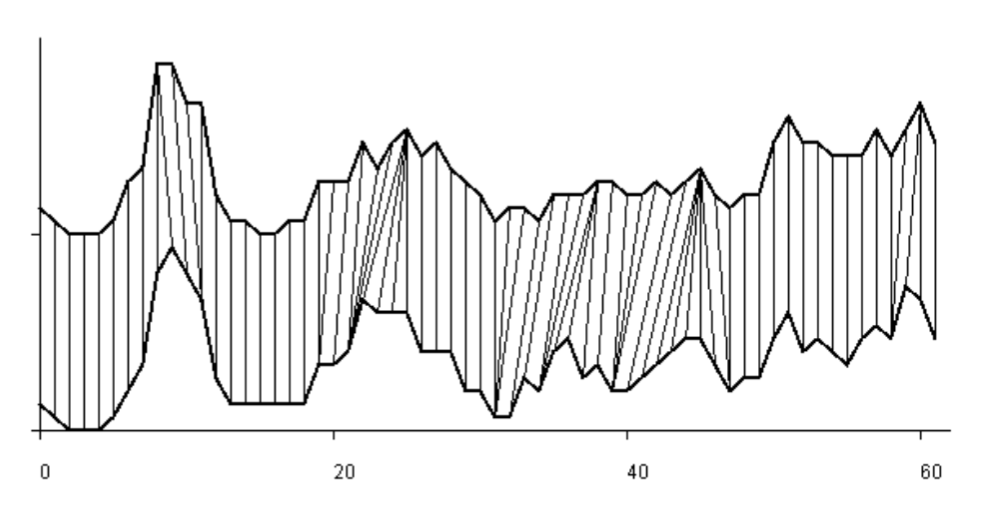
\includegraphics[width=0.7\textwidth]{DTW_1}
        \caption{Dynamic Time Warping (DTW)}
        \label{fig:DTW_1}
    \end{figure}

    Dynamic Time Warping (DTW) \cite{ref1} is a well-known algorithm for measuring similarity between two sequences, 
    which may vary in time or speed.
    It is particularly effective for sequences that are misaligned in the time dimension. 
    DTW works by finding an optimal alignment between two sequences by minimizing the cumulative distance. 
    The algorithm uses a distance matrix, which is $TDM$ in our model, where each element $(i, j)$ 
    represents the distance between the $i-th$ element of the first sequence and the $j-th$ element of the second sequence. 
    The goal is to find a path through this matrix that minimizes the total distance while respecting the ordering of the elements. 
    This path, known as the warping path, allows for stretching and compressing of the sequences to achieve the best alignment.
    The DTW distance is then the sum of the distances along this optimal path.

    With parameter $S_1 := Sequence \hspace{0.1cm} length \hspace{0.1cm} of \hspace{0.1cm} Doc1, \hspace{0.1cm} S_2 := Sequence \hspace{0.1cm} length \hspace{0.1cm} of \hspace{0.1cm} Doc2,$

    \noindent \rule{\linewidth}{0.2mm}
    \noindent $DTW \hspace{0.2cm} optimal \hspace{0.2cm} problem$:
    \begin{gather}
        DTW = \min \sum_{k = 1}^{K} l_{k} \label{eq:DTW} \\
        s.t. 
        \left\{
        \begin{array}{ll}
            l_{1} = (1,1) \\
            l_{K} = (S_1,S_2) \\
            Given \hspace{0.1cm} l_{k} = (s_1, s_2), \hspace{0.1cm} then \hspace{0.1cm} l_{k + 1} = (s_1', s_2') \hspace{0.1cm} with \hspace{0.1cm} 0 \leqslant s_1' - s_1 \leqslant 1 \hspace{0.1cm} and \hspace{0.1cm} 0 \leqslant s_2' - s_2 \leqslant 1.
        \end{array}
        \right. \\
        where \hspace{0.1cm} (s_1, s_2) := distance(s_1, s_2) = TDM(TOPIC_{Doc1 \hspace{0.05cm} on \hspace{0.05cm} s_1}, \hspace{0.05cm} TOPIC_{Doc2 \hspace{0.05cm} on \hspace{0.05cm} s_2}) \label{eq:DTW_distance}
    \end{gather}
    \noindent \rule{\linewidth}{0.2mm}

    DTW is the sum of the distances between the corresponding elements of the two sequences. 
    However, because DTW is not normalized, it increases with document length, 
    even though document similarity is not necessarily related to document length. 
    Therefore, we need to normalize DTW. There are some ways to do this, for instance, $DTW_{standard} = \frac{\sqrt{DTW}}{K}$.
    We now use \eqref{eq:DTW_standard} to normalize DTW.
    \begin{gather}
        DTW_{standard} = \frac{DTW}{K} \label{eq:DTW_standard}
    \end{gather}

    So, for the final document distance calculation, 
    we use DTW to process the topic sequence information of the documents. 
    This approach allows us to consider the overall word order, 
    thereby making the calculation of document similarity more accurate.
}

\subsubsection{Map document distance to similarity}
{
    Since the distance between documents is a value in $[0, +\infty)$, 
    while document similarity is a value in $[0, 1]$, we need to map the distance to similarity. 
    In previous research, there is no standardized method for converting document distance to similarity, 
    so we have developed our own approach.

    Obviously, all normalized DTW distances are less than the maximum entry in the $TDM \hspace{0.1cm} matrix$, 
    which we can observe once the $TDM \hspace{0.1cm} matrix$ is obtained. Based on this observation, 
    we narrow the range of document distances to be $[0, \max_{i,j} \{TDM_{i, j}\})$.

    Therefore, we can design an activation function to perform this mapping. 
    For example, taking both linear and nonlinear relationships into consideration, 
    the similarity between document A and document B can be calculated as follows:
    \begin{gather}
        Sim_{A, B} = - \alpha \times DTW_{standard}^{A, B} + 1 + e^{- \beta \times DTW_{standard}^{A, B}}
    \end{gather}

    Finally, when new documents come, we can use the whole process mentioned in chapter 4.2 to calculate 
    the similarity between them.
}
\newpage

\section{Experiments}
\subsection{Data preprocessing}
{
    We use a legal document dataset, 
    consisting of 144 legal documents and an accompanying Excel file with 100 expert-annotated similarity scores.
    We first read in the text documents.
    And then we used NLTK for tokenization, stop word removal, and stemming.
    Since sentence-level data is also required for comparison experiments, 
    we used Spacy to perform sentence segmentation on the texts. 
    All the processing results are stored, indexed by the file names.
}

\subsection{Set up}
\subsubsection{Model training}
{
    The training process for our model involved several key steps to ensure the accuracy and effectiveness of our document similarity measurements. 
    Initially, we constructed a dictionary from the training data, which included reading the text content of each document and storing it in a list. 
    This list was then converted into a bag-of-words model using the dictionary. To capture the thematic structure of the documents, 
    we trained an LDA model. If the model had not been preloaded, we trained it with 20 topics over 40 passes, ensuring robust topic modeling. 
    The model was saved for future use. Additionally, we trained a Word2Vec model on the same text data to generate word embeddings,
    which capture semantic relationships between words. This training was conducted with a vector size of 50, 
    a window size of 10, and other specified parameters. 
    Both the LDA and Word2Vec models were trained using a fixed random seed to ensure reproducibility, 
    and the training times for each model were recorded.
}

\subsubsection{Obtaining Topics}
{
    \begin{enumerate}
        \item {Token-Level Topic Probabilities:}{
            For each document, we processed the text content to determine the topic probabilities for each token. 
            Initially, each token was converted into its bag-of-words (BOW) representation using the previously constructed dictionary. 
            We then applied the trained LDA model to obtain the topic distribution for each token. 
            This distribution included probabilities for all topics, ensuring comprehensive topic coverage. 
            The results were simplified by storing only the probabilities of each
            topic for every token and identifying the most probable topic for each token.
        }
        \item {Sentence-Level Topic Probabilities:}{
            For sentence-level analysis, we adopted two methods to determine the topic probabilities: 
            averaging the token topic distributions within a sentence or directly obtaining the topic distribution for the entire sentence.
            In our current approach, we used the second method, which involved applying the LDA model to get the topic distribution for each sentence. 
            This method provided a straightforward way to capture the dominant topic for each sentence by identifying the topic with the highest probability.
        }
    \end{enumerate}

    All processing results were stored in a structured format, indexed by document identifiers, facilitating efficient retrieval and further analysis.
}

\subsubsection{Methods of measuring document similarity}
{
    In this study, we employed several methods to calculate document similarity, with a primary focus on Dynamic Time Warping (DTW). 
    The process involves computing a similarity score between two documents by 
    leveraging their topic distributions at either the token or sentence level.
    \begin{enumerate}
        \item {TS-DS on token level:}{
            This method is our PRIMARY FOCUS. 
            We used the DTW algorithm to calculate the similarity score between two documents through 
            the token-level topic distributions. 
        }
        \item {TS-DS on sentence level:}{  
            We used the DTW algorithm to calculate the similarity score between two documents through 
            the sentence-level topic distributions.
            We obtain the sentence-level topic distributions by giving the LDA model the sentence as a
            ducument. The model will return the topic distribution of the sentence.
            In this method, we also use TS-DS as method 1.
        }
        \item {TF-IDF and cosine similarity:}{
            We utilize the TF-IDF model to characterize the entire dataset, 
            obtaining representations for each document. 
            Subsequently, we employ cosine similarity to compute the similarity between every pair of documents.
        }
        \item {Document topic distribution similarity:}{
            We employ the LDA model to model the entire dataset, 
            obtaining topic distribution representations for each document. 
            Subsequently, we utilize cosine similarity to calculate the similarity between every pair of documents.
        }
    \end{enumerate}
}

\subsection{Evaluation}
{
    We conduct experiments using the four models mentioned above, 
    recording all obtained similarities. 
    Subsequently, we evaluate the accuracy of each method by comparing the obtained 
    similarities with those provided by experts using the following three metrics \eqref{eq:rmse}, \eqref{eq:f1}, \eqref{eq:corr}.

    \begin{enumerate}
        \item {RMSE:}{
            \begin{gather}
                RMSE = \sqrt{\frac{1}{100} \sum_{i=1}^{100} (Sim_{i} - Sim_{i}^{*})^2} \label{eq:rmse}
            \end{gather}
        }
        \item {F1-score:}{
            \begin{gather}
                F1-score = \frac{2}{\frac{1}{P} + \frac{1}{R}} \label{eq:f1}
            \end{gather}

            \qquad $P$ is the precision and $R$ is the recall in classification problem.

            \qquad For both predicted and expert-provided similarities, 
            we convert them into binary variables: 
            similarities greater than or equal to 0.5 are represented as 1, indicating similarity, 
            while those less than 0.5 are represented as 1, indicating dissimilarity, 
            following the approach outlined in \cite{ref3}.
        }
        \item {Correlation:}{
            \begin{gather}
                Correlation = \frac{COV(Sim, Sim^{*})}{std(Sim) \times std(Sim^{*})} \label{eq:corr}
            \end{gather}
        }
    \end{enumerate}

    The effects of all methods are showed in table \nameref{tab:effects},
    To enhance authenticity, you can see the result in Figure \ref{fig:Result} which recorded 
    the experimental results in log file with time.

    \begin{table}[htbp]
        \captionsetup{position=top, skip=8pt}
        \caption{The effects of all methods}
        \centering
        \begin{adjustbox}{width=0.9\textwidth}
            \begin{tabular}{c|c|c|c}
                \hline
                \textbf{\small Method} & \textbf{\small RMSE} & \textbf{\small F1-score} & \textbf{\small Correlation}  \\
                \hline
                \small TS-DS on token level & \small 0.3253 & \small 0.7156 & \small 0.5619  \\
                \hline
                \small TS-DS on sentence level & \small 0.2506 & \small 0.7551 & \small 0.5442    \\
                \hline
                \small TF-IDF and cosine similarity & \small 0.2185 & \small 0.6923 & \small 0.7056      \\
                \hline
                \small Document topic distribution similarity & \small 0.3448 & \small 0.8224 & \small 0.6219     \\
                \hline
            \end{tabular}
        \end{adjustbox}
        \label{tab:effects}
    \end{table}

    Although the performance of TS-DS on the token level did not surpass 
    the document topic distribution similarity model, 
    it exhibited similar effectiveness to the baseline model and outperformed the other two models. 
    This is acceptable considering that the model is still under development. 
    There are numerous aspects in which this model can be further improved, 
    which we will elaborate on in the Future Work section.
    \begin{figure}[htbp]
        \captionsetup{position=bottom, skip=8pt}
        \centering
        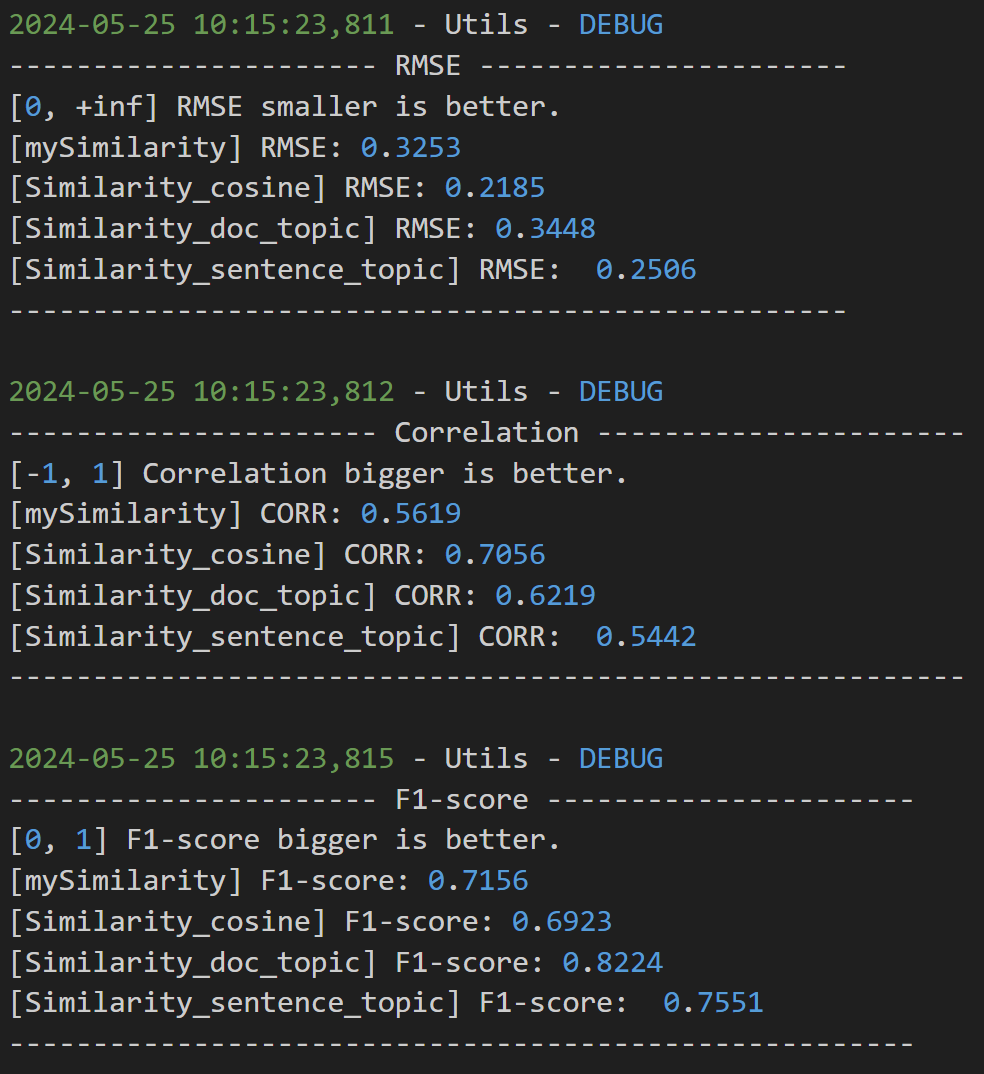
\includegraphics[width=0.6\textwidth]{result}
        \caption{Result}
        \label{fig:Result}
    \end{figure}
}
\newpage

\section{Conclusion}
{
    The cornerstone of this research is the introduction of an innovative approach to measuring text similarity that fully 
    embraces the sequential nature of text information. Traditional methods in the domain of Natural Language Processing (NLP), 
    such as the Bag-of-Words (BoW) model, have frequently neglected the importance of word order, 
    resulting in less accurate similarity assessments. Even advanced models like Word2Vec, 
    while capturing local context and some order information through its predictive framework, 
    often fall short of considering the global sequence of words across entire documents.

    Our methodology leverages text representation techniques like Word2Vec 
    to transform text into word or sentence representation vectors. 
    And We employ Latent Dirichlet Allocation (LDA) to uncover the latent topics within the document collection,
    This topic modeling provides a structured way to consider the content of texts as series.

    Building upon the word embeddings and topic distributions, 
    we introduce Word Mover's Distance (WMD) to quantify the thematic divergence between topics.       
    WMD creatively represents topics as probability distributions of words and calculates the minimum 
    work required to transform one distribution into another, 
    thus providing a measure of semantic and thematic distance that respects the order of words.

    By viewing these vectors through a time series perspective and applying Dynamic Time Warping (DTW), 
    we have developed a method that preserves the order of words and sentences, 
    thereby providing a more nuanced and precise measurement of text similarity.

    The results of our unsupervised experiments, conducted on a legal document dataset with expert-annotated similarity scores, 
    demonstrate the effectiveness of our model. Our approach, which integrates the strengths of 
    Word2Vec, WMD, and LDA with the alignment capabilities of DTW, 
    shows a strong correlation with human judgments and outperforms traditional methods that do not account for the sequential nature of text.

    The innovative aspect of our approach is the application of DTW to text similarity, 
    which effectively incorporates the sequence of words. 
    This offers a more comprehensive understanding of the thematic and semantic relationships within texts.

    In conclusion, by developing a methodology that combines the local insights of Word2Vec with the global perspective of WMD and LDA, 
    followed by the sequence alignment of DTW, we have created a comprehensive framework that 
    captures the intricate order and arrangement of words within texts. 
    This innovation is poised to enhance text analysis across a variety of NLP applications, 
    offering a more accurate and nuanced understanding of text similarity.
}
\newpage

\section{Future Work}
{
    As we look towards enhancing the accuracy and efficiency of our text similarity measurement model, 
    several promising avenues for future research and development present themselves:

    Latent LSTM Allocation \cite{ref11}: We aim to explore the integration of Latent LSTM Allocation to 
    improve the accuracy of our current topic modeling. 
    This method may offer a more nuanced understanding of the temporal dynamics within documents, 
    capturing the evolution of topics over time.

    Advanced Topic Sequence Extraction: Rather than simply taking the most probable topic for each word to extract sequence information, 
    we can apply a more sophisticated approach that utilizes WMD to 
    dynamically calculate distances between sequences at each position. 
    Although computationally intensive, this method could preserve more of the semantic information within the documents.

    Leveraging Large Language Models for Embeddings: The advent of large pre-trained language models like 
    BERT provides an opportunity to obtain more contextually rich word embeddings. 
    We plan to experiment with these models to calculate word distances, 
    potentially leading to a more accurate representation of semantic relationships.

    Custom DTW Model for Document Sequences: To better align with our model's needs, 
    we intend to design a specialized version of the DT algorithm that is tailored for comparing document sequences. 
    This could involve adapting the cost function to account for the unique characteristics of textual data.

    Supervised Learning Approach: We are considering the development of a supervised learning model 
    that can be trained on a labeled dataset to fine-tune our similarity measurement parameters. 
    By segmenting our data and employing techniques such as cross-validation, 
    we can iteratively improve our model's predictive accuracy.

    Refining DTW Distance to Similarity Mapping: The method of converting DTW distances into similarity scores warrants further investigation.
    We plan to experiment with various activation functions and hyperparameter tuning to optimize this conversion process.

    Application to Diverse Datasets: To strengthen the validation of our model, we will apply it to a wider range of datasets. 
    This will not only test the model's versatility but also help refine our approach based on diverse textual content.

    Performance Optimization: Given the computational complexity of our approach, 
    particularly with the introduction of WMD in sequence extraction and the potential use of large language models, 
    performance optimization will be a critical focus. 
    This may involve algorithmic enhancements and the exploration of parallel processing techniques.

    Integration with Information Retrieval Systems: Finally, we aim to integrate our text similarity model with information retrieval systems, 
    enhancing their ability to deliver more relevant search results and improve user experience.

    By pursuing these avenues of research, 
    we are confident that our text similarity measurement model will become an 
    even more powerful tool for applications across Natural Language Processing.
}
\newpage

\begin{thebibliography}{99}

    \bibitem{ref1} Matuschek, M., Schlüter, T., \& Conrad, S. (2008). Measuring text similarity with dynamic time warping. Proceedings of the 2008 International Symposium on Database Engineering \& Applications - IDEAS ’08, 263. \url{https://doi.org/10.1145/1451940.1451977}

    \bibitem{ref2} Mikolov, T., Chen, K., Corrado, G., \& Dean, J. (2013). Efficient Estimation of Word Representations in Vector Space (arXiv:1301.3781). arXiv. \url{https://doi.org/10.48550/arXiv.1301.3781}

    \bibitem{ref3} Bhattacharya, P., Ghosh, K., Pal, A., \& Ghosh, S. (2022). Legal case document similarity: You need both network and text. Information Processing \& Management, 59(6), 103069. \url{https://doi.org/10.1016/j.ipm.2022.103069}

    \bibitem{ref4} Salton, G., Wong, A., \& Yang, C. S. (1975). A vector space model for automatic indexing. Communications of the ACM, 18(11), 613–620. \url{https://doi.org/10.1145/361219.361220}

    \bibitem{ref5} David M Blei, Andrew Y Ng, and Michael I Jordan. 2003. Latent dirichlet allocation. Journal of machine Learning research, 3(Jan):993–1022.

    \bibitem{ref6} Kusner, M., Sun, Y., Kolkin, N., \& Weinberger, K. (2015). From Word Embeddings To Document Distances. Proceedings of the 32nd International Conference on Machine Learning, 957–966. \url{https://proceedings.mlr.press/v37/kusnerb15.html}

    \bibitem{ref7} Devlin, J., Chang, M.-W., Lee, K., \& Toutanova, K. (n.d.). BERT: Pre-training of Deep Bidirectional Transformers for Language Understanding.

    \bibitem{ref8} H.Gomaa, W., \& A. Fahmy, A. (2013). A Survey of Text Similarity Approaches. International Journal of Computer Applications, 68(13), 13–18. \url{https://doi.org/10.5120/11638-7118}

    \bibitem{ref9} Gong, H., Sakakini, T., Bhat, S., \& Xiong, J. (2018). Document Similarity for Texts of Varying Lengths via Hidden Topics. In I. Gurevych \& Y. Miyao (Eds.), Proceedings of the 56th Annual Meeting of the Association for Computational Linguistics (Volume 1: Long Papers) (pp. 2341–2351). Association for Computational Linguistics. \url{https://doi.org/10.18653/v1/P18-1218}

    \bibitem{ref10} Zhu, H. (n.d.). On Information and Sufficiency.

    \bibitem{ref11} Zaheer, M., Ahmed, A., \& Smola, A. J. (2017). Latent LSTM Allocation: Joint Clustering and Non-Linear Dynamic Modeling of Sequence Data. Proceedings of the 34th International Conference on Machine Learning, 3967–3976. \url{https://proceedings.mlr.press/v70/zaheer17a.html}

    % just for future
    \bibitem{ref12} Deshpande, A., Jimenez, C. E., Chen, H., Murahari, V., Graf, V., Rajpurohit, T., Kalyan, A., Chen, D., \& Narasimhan, K. (2023). C-STS: Conditional Semantic Textual Similarity (arXiv:2305.15093). arXiv. \url{https://doi.org/10.48550/arXiv.2305.15093}

    \bibitem{ref13} Al-Rfo+u, R., Perozzi, B., \& Skiena, S. (2014). Polyglot: Distributed Word Representations for Multilingual NLP (arXiv:1307.1662). arXiv. \url{https://doi.org/10.48550/arXiv.1307.1662}

\end{thebibliography}

\end{document}